 
\documentclass[11pt,a4paper,italian,twoside,openright]{book}

\usepackage[italian]{babel}
\usepackage[utf8]{inputenc}
\usepackage{color}
\usepackage{xcolor}
\usepackage{hyperref}
\usepackage[all]{hypcap}
\usepackage{ifthen}
\usepackage{wrapfig}
\usepackage[top=3.5cm,bottom=3.5cm,left=2.5cm,right=2.5cm,bindingoffset=1cm,]{geometry}
\usepackage{graphicx}
\usepackage{setspace}
%\usepackage{indentfirst}
\usepackage{textcomp}
\usepackage{fancyhdr} %pacchetto per le intestazioni





\DeclareGraphicsExtensions{.jpg,.png}

\newcommand{\titolotesi}{GESTIONE DELLA COMUNICAZIONE TRA CLIENTI E OPERATORI COMMERCIALI IN UN SISTEMA CRM}

%\setlength{\headheight}{3cm} %settato grandezza header...in altre parole, quanto distanzio il doc dall'intestazione
\author{Piero Bizzotto}

\pagestyle{fancy}
\linespread{1.5} %interlinea 1.5

\fancyhead{} %clear default layout
\fancyfoot{}
%\fancyhead[LE,RO]{ \slshape \rightmark}
\fancyhead[LO]{\slshape \rightmark}

\fancyhead[RE]{\slshape \leftmark}
\fancyfoot[C]{\thepage}



%CREAZIONE ELENCHI NUMERATI PERSONALIZZATI
\newcounter{Lcount}
\newcounter{Rcount}
\setcounter{Lcount}{0}
\setcounter{Rcount}{0}

\newenvironment{elenconumerato}[2][ ]
{
  \begin{list}{#1\arabic{Lcount}.}
    {
	\setcounter{Rcount}{\value{Lcount}}
	\setcounter{Lcount}{0} 
	\usecounter{Lcount} 
\addtolength{\leftmargin}{#2pt}
	}
}
{
  \end{list}
 \setcounter{Lcount}{\value{Rcount}}
}

%CREAZIONE ELENCHI PUNTATI
\newenvironment{elencopuntato}[1][]
{
\begin{list}{\textbullet} %\itemindent=#1pt
	{
	\addtolength{\leftmargin}{#1pt}
	}
} 
{
\end{list}
}


\newenvironment{elencodescrittivo}[1][]{\begin{description} \setlength{\itemindent}{#1pt} \addtolength{\leftmargin}{#1pt}} {\end{description}}

\newcommand{\TITOLODOC}{Titolo}

%footer centrale
%\cfoot{ \TITOLODOC \\  E-mail:    \href{ mailto:piero.bizzotto@gmail.com}{ piero.bizzotto@gmail.com}  }

%INSERIMENTO IMMAGINI
\newcommand{\imagerealsize}[1]{\vspace{20pt} \includegraphics{#1} }
\newcommand{\imageadapted}[1]{\vspace{20pt} \includegraphics[width=1\textwidth]{#1} }

\newcommand{\glosspath}{.\glossario}
\newcommand{\gloss}[1]{\hyperref{\glosspath~\glossario.pdf}{}{#1}{#1}}

\hypersetup{
    %bookmarks=true,         % show bookmarks bar?
    %unicode=false,          % non-Latin characters in Acrobat’s bookmarks
	%pdftoolbar=true,        % show Acrobat’s toolbar?
	%pdfmenubar=true,        % show Acrobat’s menu?
    %pdffitwindow=true,      % page fit to window when opened
    %pdftitle={My title},    % title
    %pdfauthor={Author},     % author
    %pdfsubject={Subject},   % subject of the document
    %pdfnewwindow=true,      % links in new window
    %pdfkeywords={keywords}, % list of keywords
    colorlinks=true,         % false: boxed links; true: colored links
    linkcolor=black,           % color of internal links
    %citecolor=green,        % color of links to bibliography
    %filecolor=magenta,      % color of file links
    urlcolor=teal    % color of external links
%	linktocpage=false;
}


%COLORAZIONE TESTO
\newcommand{\blue}[1]{{\color {blue} #1}} 
\newcommand{\red}[1]{{\color {red} #1}}
\newcommand{\green}[1]{{\color {green} #1}}
\newcommand{\sezione}[1]{\leftskip=0pt \section{#1} \leftskip=18pt}
\newcommand{\subsezione}[1]{\leftskip=18pt \subsection{#1} \leftskip=36pt}
\newcommand{\subsubsezione}[1]{\leftskip=36pt \subsubsection{#1} \leftskip=54pt}
\newcommand{\subsubsecindent}{54}
\newcommand{\subsecindent}{36}
\newcommand{\secindent}{18}
\newcommand{\normindent}{8}
\newcommand{\code}[1]{{\bfseries \texttt{#1}}}
\newcommand{\paragrafo}[1]{\leftskip=36pt \paragraph{#1} \leftskip=54pt}
\newcommand{\subparagrafo}[1]{\leftskip=54pt \subparagraph{#1} \leftskip=72pt} %BASE!!!
\usepackage{multirow}
\begin{document}

\begin{titlepage}
\vspace{20pt}

\begin{center}

\includegraphics[scale=0.7]{images/logo_uni}
\end{center}

\vspace{20pt}
\begin{center}

\begin{LARGE}\textsc{Universit\` a degli Studi di Padova}\end{LARGE}
\end{center}

\begin{center}
\textbf{\textsc{FACOLT\` A DI SCIENZE MATEMATICHE, FISICHE E NATURALI}}
\end{center}

\begin{center}
	\begin{large}
		\textbf{Corso di Laurea in Informatica}
	\end{large}
\end{center}

\vspace{30pt}

\begin{center}
	\begin{Large}
			\textbf{GESTIONE DELLA COMUNICAZIONE}
	\end{Large}
\end{center}			

\begin{center}
	\begin{Large}
			\textbf{TRA CLIENTI E OPERATORI COMMERCIALI}
	\end{Large}
\end{center}		


\begin{center}
	\begin{Large}
				\textbf{ IN UN SISTEMA CRM}
	\end{Large}
\end{center}		
\vspace{50pt}

\begin{center}
	\textbf{Tesi di Laurea in Informatica}
\end{center}

\vspace{30pt}

\begin{center}
\textbf{Relatrice:   \hspace{230pt}  Laureando:   \linebreak 
Prof. Ombretta Gaggi \hspace{144pt} Piero Bizzotto}
\end{center}

\vspace{30pt}

\begin{center}
\textbf{Anno Accademico 2008/09}
\end{center}

\end{titlepage}
\newpage

\clearpage
\null
\thispagestyle{empty}
\clearpage
\frontmatter
%\clearpage{\pagestyle{empty}\cleardoublepage

%\parindent=18pt %settato indentazione di default 

%\thispagestyle{fancy}
\tableofcontents
%\thispagestyle{fancy}

%\parskip=-5pt

%\sezione{Sommario} %SEZIONE SOMMARIO
%Questo documento si prefigge di relazionare l'attivit\` a di stage da me svolta
%come previsto dal corso di Laurea, e sostenuta nel periodo compreso tra l' 11
%maggio 2009 e il 3 luglio 2009 presso l'azienda TecnoBit SRL con sede a Bassano
%del Grappa(VI). Sebbene lo stage sia durato 11 settimane la durata effettiva in
%ore ha di poco superato le 300, in quanto, grazie alla disponibilit\`a
%dell'azienda ospitante ho potuto seguire le lezioni assentandomi dall'ufficio
%due mattine ogni settimana per la durata delle lezioni. Questa relazione \`e
%strutturata in quattro parti che forniscono il resoconto e l'analisi della mia
%esperienza durante lo stage. Nella prima di queste parti dar\` o una breve
%panoramica sull'ambito in cui opera TecnoBit, soffermandomi maggiormente sugli
%aspetti che ho potuto vedere di persona. Oggetto della seconda parte sar\` a il
%progetto a cui ho partecipato, e questo, per fornire una visione globale di tale
%progetto e capire da che tipo di esigenze nasce e che requisiti impliciti porta
%con s\'e. Nella terza parte invece racconter\` o lo stage stesso partendo dalla
%pianificazione iniziale e dai requisiti, per passare poi alla descrizione di
%alcune soluzioni adottate e di come queste soddisfano i requisiti. Per
%concludere, la sezione conterr\` a un consuntivo sul mio lavoro e un confronto
%con la pianificazione iniziale. L'ultima parte di questa relazione conterr\` a
%le mie conclusioni personali su questa esperienza di stage, un resoconto delle
%conoscenze acquisite e la mia visione del corso di laurea che sto terminando in
%funzione delle impressioni che ho avuto del mondo del lavoro.

%\thispagestyle{empty}
\mainmatter

%\clearpage{\pagestyle{empty}\cleardoublepage
\chapter{Presentazione dello Stage}
\section{Introduzione}
Questo documento descrive il lavoro svolto durante la mia attivit\` a di stage
presso la ditta Tecnobit S.r.l., sottolineando gli aspetti di interesse e
descrivendo in modo pi\` u rapido gli aspetti meramente tecnici. Sono venuto a
conoscenza dello stage durante \textit{Stage-IT}, evento organizzato
dall'Universit\` a degli Studi di Padova e dalla Camera di Commercio di Padova,
e dopo il colloquio tenuto con il titolare, ho capito subito quanto la mia
attivit\` a sarebbe stata utile per la ditta, che altrimenti avrebbe dovuto
attendere ancora per l'avviamento del progetto in corso, ed inoltre un sistema
informativo basato sul web era per me un argomento di grande interesse. Tale
progetto consisteva nella realizzazione di due moduli ben definiti di questo
sistema, un software web con mansioni di CRM. Gli obiettivi dello stage erano di
sfruttare il database riscritto da zero lo scorso anno da altri
\textit{stageurs} per la creazione delle sezioni di gestione interna delle
richieste provenienti da potenziali clienti, come downloads di versioni
dimostrative, richieste di DVD ecc. e l'interfacciamento del sistema con il
software VOIP utilizzato dall'azienda per la gestione delle chiamate e dei fax,
che era in precedenza minimamente integrato. Vedremo come tali obiettivi
siano stati raggiunti. Il primo capitolo introduce il contesto in cui lo
stage si \` e svolto, presenta concisamente l'azienda e fornisce le basi
necessarie alla comprensione degli obiettivi prefissati. Il secondo capitolo
invece illustra la situazione all'inizio dello stage, i problemi rilevati ed il
progetto proposto, presentandone motivazioni, punti critici, scopi ed
aspettative.  Il terzo capitolo illustra la pianificazione del lavoro svolto,
con resoconti d'inizio e fine dell'attivit\` a.  Il quarto contiene un'analisi
dei requisiti impliciti ed espliciti ricavata nella prima parte del percorso,
con relativi diagrammi dei casi d'uso. Nel quinto capitolo viene presentata la
seconda parte del mio lavoro, nella quale si illustra la realizzazione vera e
propria dei componenti analizzati. Negli ultimi capitoli saranno presentati i
problemi riscontrati durante lo stage e le conclusioni da esso tratte, i
risultati ottenuti, le conoscenze utilizzate ed acquisite e alcune
considerazioni personali sull'esperienza.

\section{L' Azienda}
La Tecnobit S.r.l. \`e una software house di Bassano del Grappa. Nasce nel 1986
come piccola azienda senza un bisogno immediato di espansione che per \`o
qualche anno, grazie anche all'acquisizione di nuovi membri nel reparto
marketing, ha deciso di cambiare strategia, iniziando una politica di crescita
tutt'oggi in corso, che la sta portando ad essere un'azienda peso rilevante nel
proprio campo di riferimento, con sbocchi nel mercato estero. Tecnobit sviluppa
una serie di applicazioni volte ad ottimizzare l’attivit\` a dei propri clienti
in tutte le diverse attivit\`a professionali svolte dagli stessi. I prodotti di
Tecnobit risolvono infatti svariate problematiche, dalla progettazione alla
certificazione energetica, dalla gestione e sicurezza dei cantieri alla
compilazione delle parcelle. Il parco software sviluppato e ad oggi regolarmente
mantenuto, negli anni \` e diventato vasto e completo, supportato anche
dall'assistenza specializzata che la software house fornisce ai propri clienti
per la risoluzione dei problemi e per l'aggiornamento dei programmi.

\section{CRM: Customer Relationship Management}
Il concetto di Customer Relationship Management descrive un insieme di azioni di
marketing volte al mantenimento della clientela gi\` a esistente, in un ottica
di aumento della soddisfazione dello stesso che porta direttamente ad un aumento
della fedelt\` a verso l'azienda. Un'impresa che adotta tale strategia non
considera unicamente il cliente come unico elemento del mercato, ma anche
l'ambiente che lo circonda, cercando di inserirsi in esso per creare rapporti
pi\` u duraturi. Il CRM si occupa in particolar modo di trovare nuovi clienti,
aumentare i rapporti con i clienti gi\`a  acquisiti e la fidelizzazione di
quelli pi\` u promettenti, detti anche \"{}clienti di primo piano\"{}.
In questa strategia si vanno bene ad inserire i software gestionali. Utilizzare
programmi specificatamente progettati per la gestione del cliente, avendo
riguardo per le strategie orientate alla fidelizzazione, pu\` o supportare e
portare grande prodotto al CRM, se adeguatamente progettato e sostenuto. Gli
strumenti che una azienda pu\` o utilizzare possono essere: 
  \begin{elencopuntato}[\subsecindent]
  	\item forum;
    \item  knowledge base e F.A.Q. per la risoluzione dei problemi comuni;
    \item  e-mail;
    \item  call center;
    \item  strumenti per la gestione dei ticket on-line;
    \item  registro dei contatti tra l'azienda ed il cliente;
    \item storia dei pagamenti effettuati dal cliente;
    \item  risorse on-line disponibili al cliente.
  \end{elencopuntato}
Ovviamente Internet rappresenta una grande opportunit\`  a nonch\` e motore
essenziale per il supporto a tale strategia.

%\section{VoIP: Voice over IP}
%Voice over IP (Voce tramite protocollo Internet), acronimo VoIP, \` e una
%tecnologia che rende possibile effettuare una conversazione telefonica
%sfruttando una rete che utilizza il protocollo IP. Il vantaggio principale di
%questa tecnologia sta nel fatto che essa elimina l'obbligo di riservare della
%banda per ogni telefonata (commutazione di circuito), sfruttando l'allocazione
%dinamica delle risorse, caratteristica dei protocolli IP (commutazione di
%pacchetto).\linebreak 
%Fra gli altri vantaggi rispetto alla telefonia tradizionale si annoverano:

%\begin{elencopuntato}[\subsecindent]
 %   \item minori costi delle infrastrutture: quando si \` e resa disponibile una
%rete IP nessun'altra infrastruttura \` e richiesta;
  %  \item nuove funzionalit\` a avanzate;
 %   \item l'implementazione di future opzioni non richieder\`a  la sostituzione
%dell'hardware.
%\end{elencopuntato}
    
%Le conversazioni VoIP non devono necessariamente viaggiare su Internet, ma
%possono anche usare come mezzo trasmissivo una qualsiasi rete privata basata sul
%protocollo IP, per esempio una LAN all'interno di un edificio o di un gruppo di
%edifici. I protocolli usati per codificare e trasmettere le conversazioni VoIP
%sono solitamente denominati Voice over IP protocols. Uno dei vantaggi di questa
%tecnologia \` e che permette di fare leva su risorse di rete preesistenti,
%consentendo una notevole riduzione dei costi in ambito sia privato che
%aziendale, specialmente per quanto riguarda le spese di comunicazione
%interaziendali e tra sedi diverse. Una rete aziendale, infatti, pu\`o  essere
%sfruttata anche per le comunicazioni vocali, permettendo di semplificare
%l’installazione e il supporto e di aumentare il grado di integrazione di uffici
%dislocati sul territorio, ma collegati tramite l’infrastruttura di rete. La
%tecnologia VoIP introduce inoltre nuove possibilit\`a  per l’offerta del
%servizio telefonico, quali: eliminare la distinzione tra chiamate locali ed a
%lunga distanza, mantenere diversi numeri telefonici su un solo collegamento,
%salvare messaggi vocali sul proprio computer, permettere telefonate
%completamente gratuite tra utenti dello stesso fornitore. Tecnobit SRL da
%qualche anno ha adottato l'IP PBX software VOIspeed PLATFORM di Harpax SRL, un
%%centralino evoluto che mette a disposizione in una soluzione unica i servizi
%della telefonia IP e la flessibilit\` a del software, consentendo una semplice
%gestione di telefonata in entrata e in uscita anche utilizzando pi\` u numeri di
%telefono interni all'azienda, cos\` i come i fax in arrivo e inviati.

%\clearpage{\pagestyle{empty}\cleardoublepage
\chapter{Contesto e ambito del progetto proposto}
\section{Sviluppo e finalit\` a dell'attuale sistema informativo}

Nello svolgimento delle proprie attivit\`a l'azienda si appoggia ad un sistema
informativo interno che gestisce i dati di interesse principali, per ottimizzare
il movimento e l'archiviazione delle informazioni e migliorare la
produttivit\`a.
Le funzioni offerte dal sistema svolgono mansioni orientate al CRM; ad ogni
cliente viene associata una scheda dati, in cui si tiene traccia di tutti i contatti con l'azienda. Oltre ai normali dati anagrafici, le
coordinate bancarie necessarie a concludere le transazioni e ai recapiti,
vengono associati al cliente anche le telefonate, email e fax inviati. Sono
conservati i dati di tutti gli acquisti effettuati dall'utente, gli
aggiornamenti e le richieste fatte al servizio di assistenza clienti.
Tecnicamente, il sistema \`e sviluppato come una web application, che esegue su
di un server LAMP. Appoggia quindi su di un database MySQL ed utilizza PHP come
motore di generazione per pagine web dinamiche. L'accesso \`e possibile
attraverso la rete, così da permettere ai dipendenti di lavorare anche dalla
loro residenza.
Tale sistema fu sviluppato internamente all'azienda ed ebbe origine da un
progetto avviato da uno studente in stage presso l'azienda, il quale ne gett\`o
le basi e ne svilupp\`o le funzioni essenziali. Quando questo sviluppatore ebbe
terminato il periodo di stage, il progetto venne lasciato in mano ai
programmatori dell'azienda i quali, negli anni, con il presentarsi di nuove
necessit\`a e il mutare delle procedure interne alla software house, ne
proseguirono lo sviluppo estendendo le funzionalit\`a esistenti e creandone di
nuove, fino a produrne
l'attuale versione. Quella di essere estremamente flessibile ed in grado di
adattarsi in fretta ai cambiamenti \`e uno dei principali requisiti per una
azienda come la Tecnobit, che da pochi anni ha cominciato ad espandersi e ad
incrementare il proprio mercato. Spesso si presenta quindi la necessit\`a di
modificare lo svolgersi di alcune procedure, o di aggiungerne di nuove. Data la
natura del sistema che, come esposto, copre e supporta gran parte delle
attivit\`a aziendali, risulta evidente come il sistema abbia, negli anni, subito
modifiche radicali ed aggiornamenti consistenti.


\section{Termini dell'attivit\` a di stage}
Nei primi incontri con l'azienda, dove \` e stata presentato lo stage e sono
stati spiegati gli obiettivi del progetto, mi \` e stata illustrata la
situazione come nel paragrafo precedente. A seguito del lavoro di altri
\textit{stageurs} lo scorso anno, i quali hanno gettato le basi per il nuovo
sistema informativo costruendone il database sottostante, rivedendo e
correggendo l'originale per aumentarne comprensibilit\` a e prestazioni,
l'azienda ha strutturato in moduli le varie parti da sviluppare per arrivare al
completamento del progetto, tra i quali appunto la gestione delle richieste
provenienti da un cliente e l'integrazione del centralino VoIP, che sono stati a
me assegnati. Il primo modulo risultava particolarmente importante in quanto
l'azienda da qualche anno ha iniziato a sfruttare intensamente le rete Internet
per l'approvigionamento di nuovi clienti, offrendo la possibilit\` a di
richiedere versioni dimostrative dei software sviluppati, intesi sia come
download, DVD da inviare, prove online, video, i quali hanno portato ad un
numero crescente nel tempo di richieste giornaliere, che sta iniziando a
diventare di difficile gestione a causa degli evidenti limiti del sistema
attuale. Il secondo modulo aveva una priorit\` a minore, ma da un'attenta
analisi delle potenzialit\` a del centralino Voip utilizzato sono emerse
funzionalit\` a che avrebbero potuto velocizzare enormemente le operazioni
svolte di routine dagli operatori commerciali dell'azienda, consentendo di
evitare passaggi macchinosi durante una telefonata ed arrivare pi\` u in fretta
a consultare i dati principali del cliente o target in quel momento al telefono.


\section{Panoramica delle tecnologie utilizzate}
La prima fase dello stage \`e stata in parte dedicata allo studio delle tecnologie da utilizzare per lo sviluppo.
Le scelte sono state fatte in base ai seguenti parametri:
\begin{itemize}
  \item complessit\`a di utilizzo: le tecnologie che richiedevano una apprendimento pi\`u approfondito per la loro 
  complessit\`a di utilizzo hanno ricevuto priorit\`a, bilanciando comunque le scelte anche secondo i bisogni stessi del
progetto da sviluppare, individuandone le funzionalit\`a necessarie;
  \item possibilit\`a di riuso del codice, per cercare di sfruttare le parti ben strutturate del vecchio sistema e adattarle se possibile al
nuovo;
  \item efficienza, in quanto questo \'e l'obiettivo cardine nello sviluppo del nuovo sistema informativo.

\end{itemize}

Le scelte quindi, in base a questi criteri sono cadute su:
\subsection{PHP, Apache e MySQL}
\textbf{PHP} \`e un linguaggio di scripting interpretato originariamente concepito per la realizzazione
 di pagine web dinamiche. Attualmente \`e utilizzato principalmente per sviluppare applicazioni web lato server ma pu\`o essere 
usato anche per scrivere script a linea di comando o applicazioni standalone con interfaccia grafica.
PHP riprende per molti versi la sintassi del C, come peraltro fanno molti linguaggi moderni, e del Perl. 
\`E fondamentalmente un linguaggio di alto livello, caratteristica questa rafforzata dall'esistenza delle sue
 moltissime API, oltre 3000 funzioni del nucleo base.
Fornisce un'API specifica per interagire con \textbf{Apache}, nonostante funzioni naturalmente con numerosi server web. 
\`E anche ottimamente integrato con il database \textbf{MySQL},un database management system (DBMS) relazionale, per il quale
 possiede pi\`u di una API. Per questo motivo esiste un'enorme quantit\`a di script e librerie in PHP, disponibili 
liberamente su Internet.
Dispone di un archivio chiamato PEAR che mette a disposizione un framework di librerie riusabili per lo sviluppo di 
applicazioni PHP e di PECL che raccoglie tutte le estensioni conosciute scritte in C.
Per motivazioni di riuso del codice gi\`a disponibile, in particolare delle ultime sezioni aggiunte di recente al sistema
informativo ancora in uso, si \`e deciso con il committente di mantenerlo come linguaggio di sviluppo, dopo aver considerato 
alternative come Perl e Python, le quali avrebbero costretto ad una riscrittura completa del codice ed avrebbero impedito anche
una eventuale parziale integrazione dei nuovi moduli con il vecchio sistema.

\subsection{CodeIgniter}
\textbf{CodeIgniter} \` e un potente framework PHP open source, creato per
permettere agli sviluppatori di avere un kit di utilit\` a semplice ed elegante,
per creare applicazioni web complete. \` E stato scelto per il progetto dopo
aver analizzato svariati frameworks quali Symfony e CakePHP, in quanto \` e
risultato di semplice utilizzo senza l'aggiunta di inutili complessit\` a, quali
l'utilizzo della linea di comando (nel caso di Symfony) o configurazioni
confusionarie, e fornisce molti strumenti che evitano l'adozione di grosse
librerie come ad esempio le PEAR, quali un ottima gestione delle sessioni,
interazione con il database sottostante (con elevate funzioni di sicurezza, come il filtro per SQL injection) 
e altre comodit\` a di un certo rilievo, e una semplice struttura logica basata sul pattern MVC, particolarmente valida
in un progetto sviluppato in team, il tutto con prestazioni superiori ai rivali
come spesso fatto notare nelle comparazioni.

\subsection{MySQL}
\textbf{MySQL} \`e  composto da un client
con interfaccia a caratteri e un server, entrambi disponibili sia per sistemi
Unix come GNU/Linux che per Windows, anche se prevale un suo utilizzo in ambito
Unix.
%\chapter{Piano di Progetto}
%\section{Pianificazione iniziale}
%\section{Modifiche al piano di lavoro}
%\section{Consuntivo}

\subsection{VOIspeed PLATFORM e VOIce Client}
\textbf{Voispeed PLATFORM} (nella sua parte server) \`e un  VOIce client IP PBX software, un centralino
evoluto che mette a disposizione in una soluzione unica i servizi innovativi
della telefonia IP e la flessibilit\`a del software, e mezzo per avere controllo
e gestione completa delle risorse telefoniche aziendali (gestione utenti,
gruppi, risponditori automatici, linee, fax).\`E inoltre una piattaforma di
comunicazione integrabile, la via per integrare ed ottimizzare tutti gli
strumenti e le tecnologie gi\`a utilizzate in azienda come DB, gestionali, CRM,
telefonia, rete dati, come \`e stato fatto appunto nel primo modulo.
\textbf{VOIce Client} invece \`e un applicativo software per postazioni PC studiato per rendere fruibili tutte le funzionalit\`a, le
informazioni e i servizi delle soluzioni PLATFORM e lavorare in sinergia con gli apparati hardware abbinabili 
(telefoni VOIspeed o cuffie), ed \`e una console operativa con cui l'utilizzatore incrementa la sua efficienza 
(accesso rapido e semplice alle funzioni con un click del mouse) e la sua capacit\`a di lavorare
in team (funzioni di conferenza, messaggi di testo, visualizzazione stato degli
interni, rubrica condivisa). In breve il portale telefonico mobile dell'utente.
L'operatore ha la possibilit\`a di essere raggiungibile al suo numero di
telefono e di continuare ad utilizzare i suoi strumenti di lavoro ovunque (fiera, ufficio, casa). 

\chapter{Analisi dei Requisiti}
La maggior parte dei requisiti sono stati raccolti in una serie di incontri con
il dott. Marco Rossi e il dott. Gianni Rossi, rispettivamente responsabile commerciale e titolare dell'azienda, 
nei quali mi sono stati esposti i principali componenti del vecchio sistema informativo, e i desideri rispetto al
nuovo, compresi i moduli in cui questo \`e stato suddiviso.

\begin{figure}[!ht]
\centering
 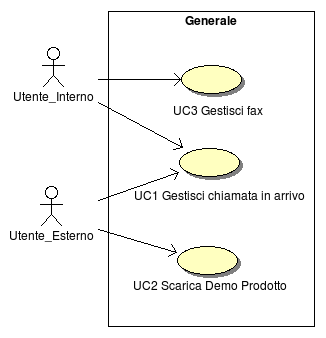
\includegraphics[scale=0.8]{./images/UC0_Generale.png}
\caption{UC0 - Generico}
\end{figure}




\section{Formazione e Studio di fattibilit\` a}
La prima e consistente parte dello stage \`e iniziata con una breve fase di formazione guidata per prendere 
conoscenza del sistema informativo in uso e dei fondamentali processi aziendali. In particolare \'e stato messo l'accento
sulle attivit\`a degli operatori commerciali, mostrandomi le varie fasi del loro lavoro, dall'acquisizione di un potenziale
 cliente fino alla sperabile vendita di uno o pi\'u prodotti, con tutti i passaggi intermedi.
Questo studio \`e stato eseguito con lo scopo di raccogliere pi\`u informazioni possibili per poter ideare un sistema 
che fosse il pi\`u possibile vicino ai bisogni dell'azienda con un occhio di riguardo verso modificabilit\'a e manutenibilit\'a, 
cosicch\'e chi dovr\` successivamente correggere o estendere il modulo sviluppato si trovi nelle condizioni ideali per farlo.
Questa prima parte di formazione dunque ha permesso una comprensione del lavoro che si sarebbe dovuto andare a realizzare. 
Durante tali incontri ho avuto modo di parlare con i rappresentanti delle aree di interesse dell'azienda, così da
poter raccogliere informazioni, suggerimenti, richieste e lamentele riguardanti ogni aspetto che il sistema informativo 
avrebbe dovuto andare a coprire. L'esperienza accumulata durante questa fase ha portato ad una visione di insieme del 
progetto, che ho cercato di rappresentare con la realizzazione di documenti che riassumevano quanto visto, 
eliminando le informazioni sovrabbondanti che non riguardassero le fasi preliminari dello sviluppo.
Un notevole supporto all'apprendimento della logica del sistema \`e venuto dalla gentile concessione dell'azienda,
 che mi ha permesso di effettuare una copia completa di tutti i codici sorgenti delle pagine PHP dell'applicazione, comprese
anche alcune pagine del sito internet, in particolare quelle riguardanti i vari prodotti e il loro download, l'accesso in 
sola lettura al database (per non rischiare di comprometterne i dati) su cui tale applicazione si appoggia, e tutto il necessario
per l'interfacciamento con il server Voispeed, per poter fare le dovute prove. 
Il modulo a me assegnato, come tutti quelli previsti, doveva basarsi su un nuovo database sviluppato da due stageurs 
lo scorso anno, che effettuarono lo studio approfondito del vecchio sistema informativo ragionando sulla possibilit\`a di 
ristrutturazione del vecchio impianto, giungendo per\`o alla conclusione che l'unica alternativa percorribile era il completo 
rifacimento del tutto, per garantire maggiore flessibilit\`a. La scelta di riscrivere il sistema ex novo comunque non 
avrebbe precluso la possibilit\`a di riutilizzare le porzioni di codice meglio realizzate: in particolare erano presenti
 numerose funzioni di recente implementazione che presentavano una buona qualit\`a del codice. 
Tali funzioni eseguivano operazioni complesse e meccaniche come la generazione delle fatture aderendo a strette regole di 
impaginazione o l'interfaccia del sistema con altri sistemi esterni che hanno necessit\`a di prelevare dati dal database. 
Riutilizzando parte del codice preesistente e adattandolo al nuovo sistema sarebbe stato possibile  
ridurre il tempo richiesto dalla noiosa implementazione di parti di poco interesse  e concentrarsi sulla 
progettazione delle nuove funzionalit\`a.

\section{Modulo VoIP e Fax}
Lo scopo principale del modulo VoIP e Fax \`e di permettere l'interazione dell'utente aziendale con il sistema
informativo per gestire tutte le operazioni effettuate di prassi durante il proprio lavoro di rapporto e comunicazione 
con il cliente. Non richiede particolari funzionalit\`a complesse, se non una semplice visualizzazione comoda e intuitiva 
dei dati del cliente chiamante/chiamato per velocizzare tutte le operazioni da eseguire per un operatore commerciale.
Inizialmente con il committente si \`e discusso sulla possibilit\'a di adozione di un nuovo software PBX, analizzando in 
particolare le soluzioni open source basate sulla piattaforma Asterisk, molto flessibili ed economiche. Nonostante le 
funzionalit\'a aggiuntive e le promesse di risparmio, una scelta cos\'i forte sarebbe stata molto complicata da effettuare, 
in quanto i benefici sarebbero stati minimi se confrontati con gli svantaggi che sarebbero sopravvenuti, in particolare per 
gli operatori che avrebbero dovuto cambiare repentinamente le loro abitudini. Siamo quindi giunti alla conclusione che fosse 
meglio studiare pi\'u a fondo le possibilit\'a proposte da Voispeed, che sono risultate sufficienti per ottenere i risultati 
prefissati.
Nella fase di analisi dei requisiti ho potuto accedere al gestionale in uso presso la ditta, in aggiunta alla possibilit\`a di 
collegarmi al centralino VoIP, tramite i quali ho potuto analizzare quali dati avessero bisogno di essere gestiti dal modulo
in procinto di essere sviluppato. Inoltre tramite alcune interviste con alcuni dipendenti ho constatato di quali strumenti
avessero bisogno per migliorare l'efficienza nel loro lavoro. Ed \`e proprio da queste interviste che sono emersi i requisiti
principali di questo modulo, in quanto l'interazione dell'applicativo VOIce Client doveva essere plasmata secondo le 
necessit\`a di questi utenti. In seguito andr\`o ad analizzare le 3 sezioni in cui \'e suddiviso il modulo.
\newpage
\subsection{Integrazione Centralino VoIP}
\begin{figure}[!ht]
\centering
 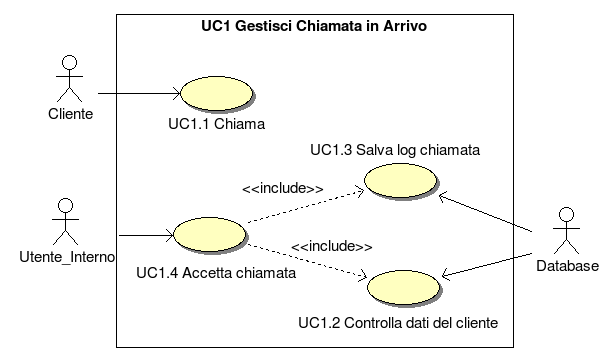
\includegraphics[scale=0.8]{./images/UC1_chiamata.png}
\caption{UC1 - Chiamata in arrivo}
\end{figure}
Le azioni della prima delle sezioni trattate sopra descritte servono ad illustrare i processi che avvengono al seguito 
dell'arrivo di una telefonata da parte di un cliente che intenda parlare con il reparto commerciale dell'azienda o con 
l'assistenza tecnica. In precedenza, per qualsiasi utente, l'unica informazione reperibile in questa fase era l'identit\`a del cliente/target chiamante, nel caso questo
fosse registrato nel database aziendale, trovata utilizzando come parametro ovviamente il numero di telefono del chiamante.
Dalle interviste effettuate, \`e emerso un bisogno generale di snellire tutte le operazioni che un commerciale era portato
ad eseguire una volta ricevuta una telefonata, che principalmente erano raccogliere i dati del cliente chiamante dal sistema informativo
tramite ricerca del nominativo, atto che portava per\'o ad uno spreco di tempo all'inizio della telefonata che in qualche caso poteva
infastidire il cliente. La necessit\'a primaria diventava quindi quella di poter ottenere pi\'u informazioni possibili all'arrivo
di una chiamata, e di poter accedere immediatamente alla scheda del cliente con tutti i dati inseriti nel database. Inoltre 
altro bisogno indispensabile risultava l'automatizzazione della procedura di inoltro di una telefonata al commerciale tutelante
del cliente chiamante, cosa che avveniva in modo del tutto privo di regole con situazioni paradossali all'interno degli uffici, come 
richieste a voce ai vicini di scrivania per stabilire a chi spettasse la telefonata.
\subsection{Invio Fax}
Il client VOIce integra una funzionalit\`a di invio fax, consentita per\'o solamente ad alcuni utenti abilitati all'invio. 
Necessit\`a degli utenti \'e di poter visualizzare l'elenco dei fax da loro inviati tramite un'apposita schermata del sistema
informativo, in modo da avere a disposizione uno storico delle loro operazioni di invio.
\subsection{Ricezione Fax}
L'amministratore del sistema o chi abbia i permessi adeguati devono poter consultare i fax arrivati in azienda tramite
apposita pagina del sistema informativo, e poter assegnarli al cliente corretto registrato nel database, non senza qualche nota
a margine in caso di necessit\`a. Se il fax arrivato riguarda un particolare commerciale, questo deve poter essere informato
 tramite un'apposita funzione, in modo che questi possa leggerlo a sua volta.
\subsection{Use Cases}
\subsection*{UC1.1 Chiama}
\subsubsection*{Attori coinvolti} Cliente esterno, Server Voispeed.
\subsubsection*{Scopo e descrizione sintetica}
Il cliente telefona alla ditta, che gestisce la telefonata tramite il software VOIP.
\subsubsection*{Flusso di eventi}
\begin{enumerate}
\item Il cliente telefona all'azienda.
\item Il centralino VOIP riceve la telefonata e si prepara ad inoltrarla.
\end{enumerate}
\subsubsection*{Precondizioni}  Il centralino \` e in attesa di una telefonata esterna.
\subsubsection*{Postcondizioni} Il centralino ha risposto e attende di sapere dal cliente il tipo di operatore con cui questi vuole parlare.

\subsection*{UC1.2 Controllo del tipo di chiamata}
\subsubsection*{Attori coinvolti} Server Voispeed.
\subsubsection*{Scopo e descrizione sintetica}
Il centralino VOIP elabora la richiesta dell'utente impostando il reparto da contattare indicatogli dal cliente (commerciale, assistenza, amministrazione).
\subsubsection*{Flusso di eventi}
\begin{enumerate}
\item Il centralino ha ricevuto la telefonata.
\item Il centralino imposta il reparto al quale passare la telefonata.
\end{enumerate}
\subsubsection*{Precondizioni} Il centralino \` e pronto a selezionare il reparto da passare al cliente.
\subsubsection*{Postcondizioni} Il centralino ha impostato il reparto desiderato dal cliente chiamante.

\subsection*{UC1.3 Inoltra ad un utente del gruppo corretto}
\subsubsection*{Attori coinvolti} Server Voispeed, utente interno.
\subsubsection*{Scopo e descrizione sintetica}
Il centralino VOIP  inoltra la chiamata al reparto indicatogli dal cliente (commerciale, assistenza, amministrazione).
\subsubsection*{Flusso di eventi}
\begin{enumerate}
\item Il centralino verifica a che reparto passare la telefonata.
\item Il centralino inoltra la chiamata all'utente interno corretto.
\end{enumerate}
\subsubsection*{Precondizioni} Il centralino \` e pronto ad inoltrare la telefonata all'utente interno corretto.
\subsubsection*{Postcondizioni} Il centralino ha inoltrato correttamente la chiamata.

\subsection*{UC1.4 Controlla dati del cliente chiamante}
\subsubsection*{Attori coinvolti} Server Voispeed, Database.
\subsubsection*{Scopo e descrizione sintetica}
Nel caso di telefonata commerciale, il client Voispeed dell'utente a cui viene inoltrata la chiamata raccoglie i dati del cliente chiamante (tramite il numero di telefono e utilizzando il database) indicando, se presenti, le indicazioni sul commerciale che ha in tutela il dato cliente, seguendo le regole del regolamento interno dell'azienda.
\subsubsection*{Flusso di eventi}
\begin{enumerate}
\item Il client Voispeed dell'operatore controlla se il cliente chiamante \` e gi\` a tutelato da un commerciale per decidere a chi inoltrare la chiamata.
\end{enumerate}
\subsubsection*{Precondizioni} Il client \`e pronto a controllare quale operatore commerciale ha sotto tutela il cliente chiamante.
\subsubsection*{Postcondizioni} Il client ha controllato i dati del cliente, se esistente, e indica all'operatore chi, se presente, tutela il cliente che sta chiamando.


\subsection*{UC1.5 Salva il log della chiamata}
\subsubsection*{Attori coinvolti} Server Voispeed, Database.
\subsubsection*{Scopo e descrizione sintetica}
Il centralino VOIP salva nel database una traccia della telefonata avvenuta.
\paragraph{Flusso di eventi}
\begin{enumerate}
\item Il centralino raccoglie i dati della telefonata.
\item Il centralino scrive nel database tali dati.
\end{enumerate}
\subsubsection*{Precondizioni} Il centralino \`e pronto a registrare i dati della telefonata.
\subsubsection*{Postcondizioni} Il centralino ha registrato nel database i dati della telefonata avvenuta.

\subsection{Requisiti}
\underline{\textbf{Funzionali}}
\begin{itemize}
 \item \textsc{Obbligatori}
	 \begin{description}
	  \item[RFO1:] Il sistema deve fornire all'utente del centralino che risponde alla chiamata tutti i dati utili riguardanti il cliente atti
a snellire le operazioni da svolgere nell'arco della chiamata.
	  \item[RFO2:] Il sistema deve permettere all'utente di utilizzare delle scorciatoie per l'accesso alle parti fondamentali del sistema operativo
tramite un solo click del mouse.
	  \item[RFO3:] Il sistema deve fornire tutte le funzioni per il trasferimento di chiamata dall'operatore commerciale che riceve la telefonata 
a quello che detiene la tutela del cliente chiamante.
\item[RFO4:] Per gli operatori del Servizio Assistenza, il sistema deve fornire all'arrivo della chiamata tutti i dati riguardanti i software 
posseduti dal cliente chiamante e la loro copertura assistenziale;
\item[RFO5:] Il sistema deve registrare i dati principali di una telefonata avvenuta come durata, numeri di telefono e date di inizio/fine;
\item[RFO6:] Il sistema deve permettere la consultazioni di tali tabulati, fornendo dei filtri per data e per utente interno;
\item[RFO7:] Il sistema deve permettere l'inserimento di un contatto telefonico solo se la telefonata relativa \'e effettivamente 
avvenuta.
\item[RFO8:] Il sistema deve consentire ad un utente che ha la possibilit\'a di inviare un fax di visionarne l'elenco totale tramite un report 
apposito;
\item[RFO9:] Il sistema deve permettere ad un amministratore di visualizzare i dati dei fax in arrivo e di poterli collegare al cliente corretto, 
con le dovute annotazioni opzionali;
\item[RFO10:] Inoltre un amministratore deve poter inoltrare un fax ricevuto all'operatore che sta seguendo la trattativa con quel cliente;

\item[RFO3:] 
 	\end{description}

\item \textsc{Desiderabili}
\item \textsc{Opzionali}


\end{itemize}

\underline{\textbf{Di Qualit\`a}}
\begin{itemize}
 \item \textsc{Obbligatori}
	 \begin{description}
	  \item[RQO1:] Il codice scritto segue le linee guida stabilite dagli stessi creatori di CodeIgniter, disponibili su 
\url{http://codeigniter.com/user_guide/general/styleguide.html}.
	  \item[RQO2:] Il codice scritto si basa sul pattern MVC.
	  \item[RQO3:] Il codice xHTML e CSS devono essere validati dagli strumenti forniti dal W3C.
	  \item[RQO3:] Il sistema deve garantire agli utilizzatori delle prestazioni velocistiche accettabili.
 	\end{description}
\item \textsc{Desiderabili}
\item \textsc{Opzionali}


\end{itemize}

\underline{\textbf{Di Interfacciamento}}
\begin{itemize}
 \item \textsc{Obbligatori}
	 \begin{description}
	  \item[RIO1:] Utilizzo del DBMS MySQL.
	  \item[RIO2:] Il codice usato per la realizzazione delle classi \`e il PHP.			
	  \item[RIO3:] Utilizzo del framework CodeIgniter.
	  \item[RIO4:] Utilizzo del web server Apache.
	  \item[RIO5:] Utilizzo del software Voispeed per la gestione delle telefonate.
	  \item[RIO6:] Il sistema informativo deve poter essere utilizzato con tutti i browser in circolazione attualmente.
	  \item[RIO7:] Il sistema deve essere facile da utilizzare: tutte le funzionalit\`a devono essere disponibili 
		      all’utente, attraverso una comoda interfaccia grafica (pulsanti, caselle per l’input degli utenti,
			combobox, checkbox, ecc).
	  \item[RIO8:] Il sistema informativo permette all’utente di visualizzare in maniera facile veloce i dati di 
		      maggior interesse mettendo a disposizione filtri e viste di vario genere, come i report dei fax e del 
		      registro delle chiamate.
 	\end{description}
\item \textsc{Desiderabili}
\item \textsc{Opzionali}


\end{itemize}



\newpage
\section{Modulo Richieste}
Il secondo modulo raggiunge un livello di complessit\`a pi\'u elevato, a causa delle numerose variabili che entrano in contatto
tra di loro. L'obiettivo in questo caso era quello di spostare la gestione delle richieste provenienti dal sito dell'azienda da
GetResponse, un software di email marketing basato sul web che offre funzionalit\`a di spedizione di newsletters e di
risposta automatica, al nuovo sistema informativo, per tenere traccia di tutte le operazioni svolte dai potenziali clienti 
interessati alle versioni dimostrative dei software sviluppati dall'azienda. 
\subsection{Gestione delle richieste}
\begin{figure}[!ht]
\centering
 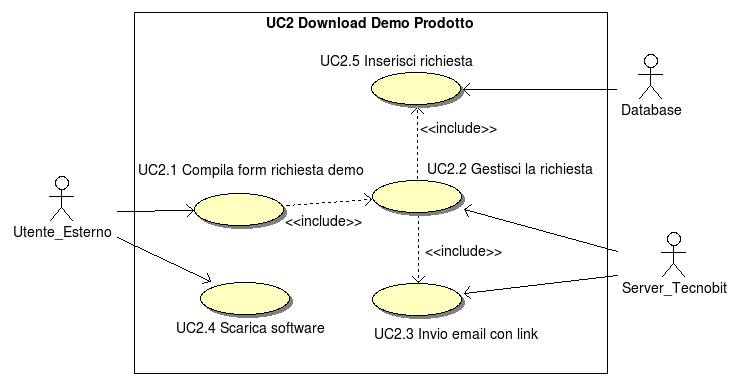
\includegraphics[scale=0.8]{./images/UC2_download.png}
\caption{UC2 - Download Versione Dimostrativa}
\end{figure}
Requisito fondamentale era quindi quello di effettuare questa transizione in modo da automatizzare tutta la gestione delle richieste
in arrivo utilizzando il sistema informativo aziendale, tracciando la fonte (che pu\`o essere un download di una versione dimostrativa
dal sito dell'azienda, l'importazione da un database di contatti regolarmente acquistato, oppure la scansione di una apposita casella
di posta elettronica dove vengono inoltrati i dati dei clienti italiani che hanno effettuato il download di una versione di prova del
software Bricscad dal sito dello sviluppatore canadese), consentendo ad un amministratore di gestire l'elenco di queste richieste
(acquisizione, assegnazione, cancellazione), e ad un utente commerciale di poterne acquisire una quantit\`a giornaliera limitata, 
seguendo un regolamento commerciale interno all'azienda.
\subsection{Use Cases}

\subsection*{UC 2.1 Compila Form Richiesta Demo}
\subsubsection*{Attori coinvolti} Utente Esterno, Server Tecnobit.
\subsubsection*{Scopo e descrizione sintetica}
L'utente esterno compila il form per scaricare un dimostrativo, richiedere un DVD o provare un programma nella sua 
versione online inserendo i propri dati personali specificando il prodotto selezionato.
\subsubsection*{Flusso di eventi}
\begin{enumerate}
\item Il cliente seleziona il prodotto del quale vuole richiedere una versione dimostrativa o altro.
\item Il cliente compila il form apposito per il download.
\end{enumerate}
\subsubsection*{Precondizioni} Il sistema ha caricato la pagina con il form per il download.
\subsubsection*{Postcondizioni} L'utente esterno ha compilato il form e ha inviato la richiesta al server.

\subsection*{UC 2.2 Gestisci la richiesta}
\subsubsection*{Attori coinvolti} Utente Esterno, Server Tecnobit.
\subsubsection*{Scopo e descrizione sintetica}
Il sistema elabora la richiesta effettuata dall'utente esterno.
\subsubsection*{Flusso di eventi}
\begin{enumerate}
\item Il cliente invia la richiesta cliccando sull'apposito tasto.
\item Il sistema elabora i dati inviati, controllando i dati del richiedente, nello specifico se \`e o no inserito nel database
dell'azienda o se si tratta di un nuovo potenziale cliente.
\end{enumerate}
\subsubsection*{Precondizioni} L'utente ha compilato il form di richiesta.
\subsubsection*{Postcondizioni} Il sistema ha gestito la richiesta dell'utente.

\subsection*{UC 2.3 Invio e-mail con link}
\subsubsection*{Attori coinvolti} Utente Esterno, Server Tecnobit.
\subsubsection*{Scopo e descrizione sintetica}
Il sistema invia una mail all'utente con il link per procedere allo scaricamento della versione dimostrativa del prodotto.
\subsubsection*{Flusso di eventi}
\begin{enumerate}
\item Il sistema raccoglie i dati dell'utente, tra i quali l'indirizzo e-mail.
\item Il sistema invia la mail con il link per scaricare la versione dimostrativa del software scelto.
\end{enumerate}
\subsubsection*{Precondizioni} Il sistema ha ricevuto i dati dell'utente.
\subsubsection*{Postcondizioni} Il sistema ha inviato il link per lo scaricamento all'utente.

\subsection*{UC 2.4 Scarica Software}
\subsubsection*{Attori coinvolti} Utente Esterno, Server Tecnobit.
\subsubsection*{Scopo e descrizione sintetica}
L'utente scarica il software scelto dal link ricevuto per email.
\subsubsection*{Flusso di eventi}
\begin{enumerate}
\item L'utente riceve la mail.
\item L'utente scarica la demo tramite il link fornitogli.
\end{enumerate}
\subsubsection*{Precondizioni} L'utente attende la mail dal sistema.
\subsubsection*{Postcondizioni} L'utente ha scaricato la versione dimostrativa del software.

\subsection*{UC 2.5 Inserisci richiesta}
\subsubsection*{Attori coinvolti}  
Database, Server Tecnobit. 
\subsubsection*{Scopo e descrizione sintetica}
Nel database vengono inseriti i dati dell'utente che ha effettuato la richiesta di download. 
\subsubsection*{Flusso di eventi}
\begin{enumerate}
\item Il sistema raccoglie i dati dell'utente.
\item Viene creata una voce nel database che descrive l'utente e l'operazione da lui effettuata, per permettere agli 
operatori commerciali di contattarli successivamente.
\end{enumerate}
\subsubsection*{Precondizioni} Il sistema gestisce la richiesta.
\subsubsection*{Postcondizioni} Il sistema ha inserito la richiesta nel database in modo da poter contattare successivamente
il cliente che l'ha effettuata.
\subsection{Requisiti}
\underline{\textbf{Funzionali}}
\begin{itemize}
 \item \textsc{Obbligatori}
	 \begin{description}
	  \item[RFO11:] Il sistema deve consentire ad un cliente di scaricare la versione dimostrativa di un prodotto tramite una semplice
pagina web.
	  \item[RFO13:] Il sistema deve inviare al cliente un' e-mail con all'interno il link per il download del demo del prodotto voluto.
	  \item[RFO14:] Il sistema deve controllare i dati del cliente che effettua la richiesta, per verificare se questo \`e gi\`a 
inserito nel database aziendale.
\item[RFO15:] Nel caso il cliente sia gi\`a inserito, ed un commerciale lo abbia in tutela per il periodo corrente, il sistema deve inviare un messaggio
a quest'ultimo per informarlo della richiesta avvenuta.
\item[RFO16:] Nel caso il cliente sia nuovo, ma proveniente da una provincia tutelata da un agente predefinito, quest'ultimo deve vedersi 
automaticamente assegnata la richiesta e inviato un messaggio per avvertirlo di questo, in modo che possa contattare il cliente il prima
possibile.
\item[RFO17:] Il sistema deve permettere all'amministratore di decidere quali richieste debbano essere visulizzabili da tutti i commerciali, 
e quali invece no.
\item[RFO18:] Il sistema deve consentire ad un commerciale di acquisire una richiesta pubblica per un numero di volte giornaliere stabilito 
a priori dall'amministratore.
\item[RFO19:] Il sistema deve permettere ad un amministratore di assegnare le richieste a piacere ad un commerciale, e avvisare ques'ultimo 
dell'assegnazione avvenuta tramite un messaggio.
\item[RFO20:] Il sistema deve provvedere a conteggiare la durata delle tutele di un cliente per un determinato utente, in modo da toglierle in 
caso di scadenza.
 	\end{description}

\item \textsc{Desiderabili}
\item \textsc{Opzionali}


\end{itemize}

\underline{\textbf{Di Qualit\`a}}
\begin{itemize}
 \item \textsc{Obbligatori}
	% \begin{description}
Valgono tutti i requisiti di questo tipo considerati per il modulo precedente.
 	%\end{description}
\item \textsc{Desiderabili}
\item \textsc{Opzionali}


\end{itemize}

\underline{\textbf{Di Interfacciamento}}
\begin{itemize}
 \item \textsc{Obbligatori}
      Valgono tutti i requisiti di questo tipo considerati per il modulo precedente.
	% \begin{description}
	    
 	%\end{description}
\item \textsc{Desiderabili}
\item \textsc{Opzionali}


\end{itemize}

\chapter{Svolgimento del Progetto: Sviluppo dei moduli}

\section{Il modello di sviluppo}
La necessit\`a di rendere il sistema estendibile e manutenibile ha richiesto l'adozione di un framework di sviluppo 
come CodeIgniter, il quale come detto si basa sul pattern architetturale MVC (Model-View-Controller) che ha come scopo
 quello di isolare la logica di business dell'applicazione dalla sua interfaccia con l'utente. Questa separazione rende 
molto pi\`u semplice la modifica della visualizzazione grafica o della logica sottostante senza dover adattare anche il
resto dell'applicazione. In MVC, il model rappresenta l'informazione e le regole necessarie per manipolarla;
 la view corrisponde agli elementi dell'interfaccia utente che hanno il compito di presentare una certa visione dei dati; 
il controller gestisce gli eventi provenienti dall'utente ed eventualmente effettua opportune azioni sul model.


\section{Progettazione e sviluppo}
Analizzati i requisiti dei moduli si \`e deciso di procedere quindi con la progettazione e lo sviluppo. In questo modo ho avuto 
la possibilit\`a di valutare la qualit\`a dell'analisi, gi\`a verificata con l'azienda, 
e di fornire un solido punto di partenza su cui ciascun modulo avrebbe potuto appoggiarsi in
modo indipendente dagli altri che saranno sviluppati da altri stageurs. Infatti, essendo l'obiettivo primario del rifacimento 
dell'intero sistema informativo la migliore efficienza, risulta conseguentemente anche la componente di
maggior delicatezza ed interesse, che quindi necessita di pi\`u tempo per poter raggiungere una forma stabile. 
Inoltre lavorare alla progettazione dei moduli seguendo l'analisi appena svolta, avrebbe permesso di valutare
se i requisiti identificati fossero sufficientemente esaustivi o se invece alcuni aspetti erano stati omessi.
\subsection{Il Database}
Le prima azione da eseguire consisteva nella ristrutturazione delle tabelle del database creato appositamente lo scorso anno.
Essendo stata fatta una progettazione il pi\`u generale possibile, si \`e visto subito che molte tabelle specifiche per i miei moduli 
erano assenti. Un primo passo obbligato \`e stato quindi quello di integrare con le nuove tabelle il database, in modo da predisporlo 
allo sviluppo.
\begin{figure}[!ht]
\centering
  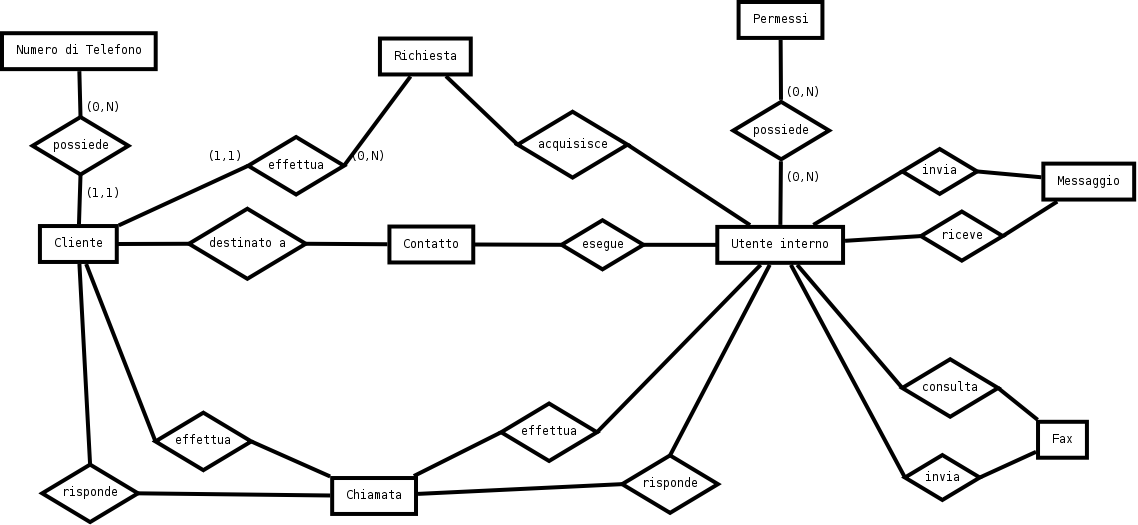
\includegraphics[scale=0.3]{./images/ER.png}
\caption{Diagramma ER del database}
\end{figure}
 
Per rappresentare il \"{}frammento\"{} di database ho scelto di un diagramma E-R, azione dettata dal contesto della progettazione
 iniziale dei database, e l'approccio scelto prevedeva di disegnare uno schema ad alto livello.
Sei sono state le entità che sono risultate evidenti come fulcro del modulo, attorno a cui ruotava la funzione delle altre entit\`a:
\begin{itemize}
  \item Cliente
  \item Contatto
  \item Utente interno
  \item Fax
  \item Richiesta
  \item Chiamata
\end{itemize}

I collegamenti tra le entit\`a cercano di racchiudere le azioni maggiormente eseguite nel contesto dei due moduli a me assegnati, come i
contatti che avvengono tra utenti interni e clienti, oppure la possibilit\`a per un cliente di avere pi\`u numeri di telefono associati.

\subsection{Il sistema informativo}
Basandosi quindi sul database appena descritto, tramite diagramma delle classi UML viene descritta una prima struttura dei modulo da 
sviluppare, con le dipendenze esistenti derivanti dalla progettazione effettuata e dal pattern MVC utilizzato.

\begin{figure}[!ht]
\label{voip}
\centering
  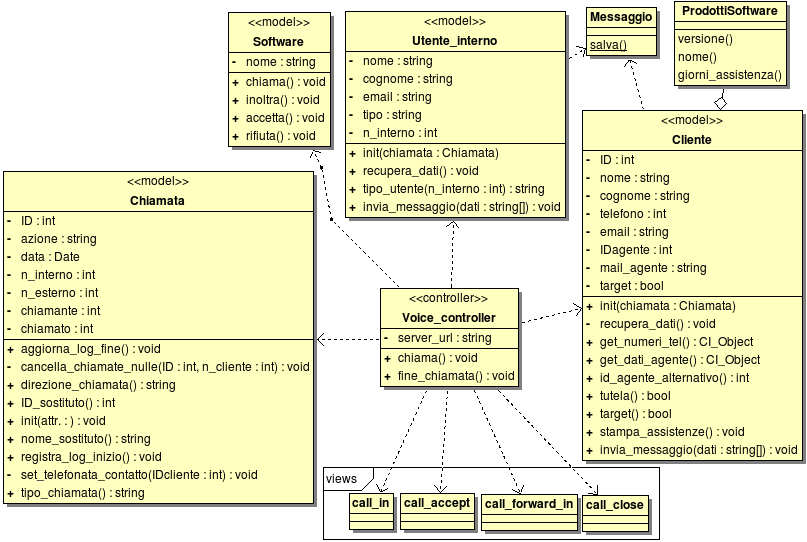
\includegraphics[scale=0.7]{./images/VoIPMVC.png}
\caption{Diagramma delle classi del modulo VoIP}
\end{figure}

Innanzitutto, dalla figura \ref{voip} si pu\`o notare come il fulcro del primo modulo sia sicuramente la \textit{Chiamata}, modello che contiene tutte le 
operazioni riguardanti una generica telefonata (in entrata o in uscita), come il salvataggio del log della chiamata.
Il controller ha il compito di raccogliere i dati di questa chiamata (per la maggior parte dall'integrazione con Voispeed) ed 
utilizzarli per chiamare le viste dedicate, a seconda dell'evento verificatosi(arrivo di una chiamata, oppure terminazione della stessa).
Le classi \textit{Cliente} ed \textit{Utente Interno}, allo stesso modo, vengono istanziate dal controller ad ogni chiamata, e 
contengono i dati principali dell'utente interno e del cliente coinvolti nella telefonata, raccogliendone i dettagli dal database, come 
ad esempio il nome del proprio sostituto nel caso di un operatore commerciale, oppure le informazioni sulla tutela di un cliente 
e i prodotti per cui quest'ultimo abbia assistenza tecnica garantita.
\textit{SoftwareProdotto} si occupa proprio della raccolta di questi dettagli, sfruttando le funzioni sviluppate da un'altro stageur, 
a cui era stato assegnato il modulo sulla gestione di un sistema per il supporto tecnico online.
In particolare, l'istanza di tale classe permette di accedere ai dati di un cliente riguardanti 
prodotti ancora in assistenza, in modo da velocizzare le operazioni svolte dai tecnici, che all'arrivo di una
chiamata riescono a conoscere in anticipo il contesto sul quale essa si baser\`a, conoscendo i prodotti posseduti dal cliente.
%La classe \textit{Log chiamate} si occupa di tenere traccia nel database di tutte le chiamate che avvengono con un cliente,
 %raccogliendo i dati principali delle stesse, come ad esempio la durata e i numeri di telefono comunicanti.
La classe \textit{Software} cerca di astrarre le operazioni svolte dal client VoIP in modo da permettere una 
futura indolore adozione di un nuovo software di questo tipo, raggruppando in metodi le normali azioni come l'accettazione, 
l'inoltro o il rifiuto di una chiamata. Questo comunque gi\`a dalle prime considerazioni fatte era apparso di difficile attuazione,
 a causa soprattutto della diversit\`a tra le API dei software, che nella maggior parte dei casi offrono funzionalit\`a magari 
simili tra loro ma implementate in modo molto diverso.

\newpage
\begin{figure}[!ht]
\label{voip}
\centering
  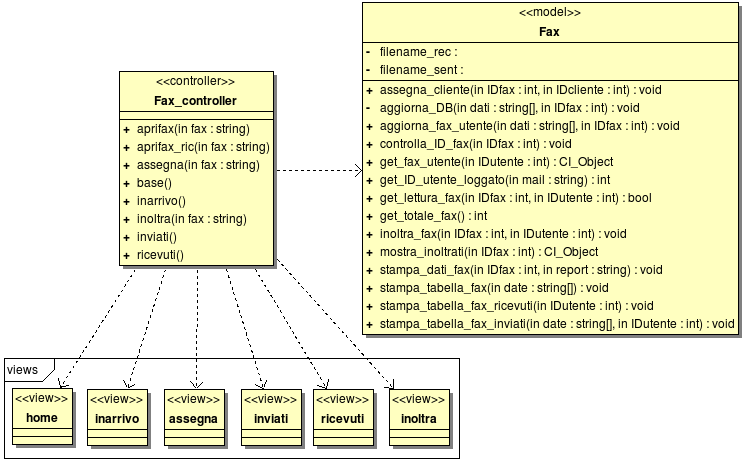
\includegraphics[scale=0.8]{./images/FaxMVC.png}
\caption{Diagramma delle classi della gestione Fax}
\end{figure}


Infine la classe \textit{Fax} gestisce tutte le operazioni effettuate sui fax, anch'essa interfacciata con \textit{Cliente} e 
\textit{Utente}, in quanto attori principali sui quali essa si basa. In particolare contiene i riferimenti ai due files di 
testo che Voispeed utilizza per tenere traccia dei fax inviati e ricevuti dal server, e tutte le varie funzioni di utilit\`a 
per la loro gestione. 
Andando ad analizzare il secondo modulo, la classe \textit{Richiesta} racchiude invece tutti i metodi per la gestione
delle richieste memorizzate nel database, come la loro assegnazione, acquisizione, importazione da fonti diverse dal download diretto 
di un demo di un prodotto. Proprio per usufruire di questa ultima possibilit\`a \`e presente la classe \textit{Form Download}, 
che controlla tutti i meccanismi riguardanti il salvataggio dei dati del cliente richiedente la versione dimostrativa, come ad 
esempio il controllo di tali dati per decidere come gestire la richiesta, oppure l'invio dell' e-mail contenente i link(utilizzando i metodi 
resi disponibili dalla classe \textit{Mail inviata}).
Come nel caso di \textit{SoftwareProdotto}, la classe \textit{Messaggio} ed in particolare il metodo \textit{salva} sono stati 
sviluppati appositamente da un altro stageur, in quanto entrambi i moduli specificati utilizzano in pi\`u occasioni i messaggi 
interni per la comunicazione tra sistema/utente, o anche utente/utente, per svariati bisogni.

\section{Realizzazione}
Verranno illustrate ora le soluzioni adottate per lo sviluppo dei due moduli, associando alla descrizione delle scelte effettuate 
alcune immagini per comprendere al meglio il contesto.
\subsection{Modulo VoIP e Fax}
Per la parte riguardante il VoIp, e quindi l'interazione con il sofware Voispeed, occorre una piccola introduzione riguardo al suo 
funzionamento. Il client infatti permette di sfruttare delle pagine web opportunamente costruite, passando come parametri mediante 
il metodo GET dell'HTML, il quale \`e usato come mezzo per l'invio dei dati come parte di un URL. 
Alla ricorrenza di un determinato evento riguardante la chiamata, \`e possibile collegare il cliente ad una pagina web e passare pi\`u
dati contemporamente, tra i quali:
\begin{itemize}
 \item !00 = proprio numero interno;
 \item !01 = numero remoto (chiamato o chiamante);
 \item !02 = azione (evento che ha attivato l'invocazione dello script e corrisponde a quelli che si possono selezionare);
 \item !05 = ID della chiamata (generato automaticamente dal Server e identifica in modo univoco la chiamata);
 \item !06 = numero chiamante originario (questo parametro indica il numero effettivo del chiamante);
 \item !07 = numero chiamato originale (questo parametro indica il numero effettivo chiamato dall'utente remoto).
\end{itemize}
  Utilizzando appunto questi parametri tramite il controller \textit{call} e la sua funzione interna \textit{chiama}, alla quale 
vengono passati ad ogni evento prestabilito nella configurazione (nella fattispecie CALL IN, CALL ACCEPT, CALL CLOSE e CALL FORWARD IN), 
\`e stato possibile richiamare le pagine corrette semplicemente tramite l'apposita istanza del browser Internet Explorer 
utilizzata dal client.
Ad esempio se arrivasse una chiamata dall'esterno dal numero 02675456 a cui rispondere per l'utente con ID=6, allora si avrebbe:
 !02=CALL IN, !06=02675456, e !07=6.
Utilizzando queste funzionalit\`a, \`e stata associata una pagina da visualizzare per ogni evento sopra descritto, che appare 
all'utente una volta che tale evento si attiva. Ad esempio, come mostrato nella figura seguente, ad una chiamata in arrivo verr\`a 
visualizzata questa finestra all'operatore commerciale:



\begin{figure}[!ht]
\centering
  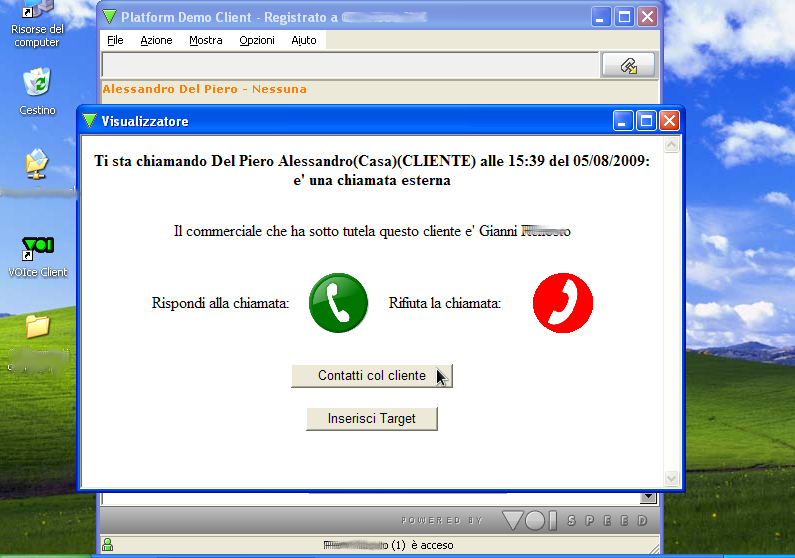
\includegraphics[scale=0.8]{./images/chiamata_commerciale.png}
\caption{Chiamata in arrivo a Commerciale}
\end{figure}

Come si pu\`o vedere, il sistema informativo controlla nel database se il numero di telefono chiamante \`e collegato ad un cliente, 
fornendone i dati utili all'operatore a cui arriva la telefonata, nel caso siano presenti. In particolare, oltre al nome e la qualifica 
del cliente, viene mostrato anche il nome dell'operatore commerciale che, nel periodo corrente, detiene la tutela esclusiva sul cliente in 
questione. Questa informazioni \`e sicuramente la novit\`a principale che riguarda questa parte, in quanto in precedenza ad ogni 
telefonata si creava una certa confusione per trovare questo dato, dovendo effettuare ogni volta una ricerca manuale nel (lento) sistema informativo 
per trovare chi, se presente, avesse il diritto alla tutela, e girare a questo la telefonata.
Questo problema viene ora aggirato fornendo a chi risponde tutte le scorciatoie necessarie ad effettuare questa procedura in modo 
semi-automatico, guidando l'utente passo passo (tramite l'utilizzo di alcune funzionalit\`a del framework javascript jQuery
\section{Test}
%\thispagestyle{empty}

\chapter{Problemi incontrati}

\chapter{Conclusioni}
\section{Risultati ottenuti durante lo stage}
\section{Conoscenze utilizzate ed acquisite}
\section{Considerazioni personali}
\clearpage{\pagestyle{empty}\cleardoublepage
\addcontentsline{toc}{chapter}{Glossario}
\chapter*{Glossario}
\section*{A}
\hypertarget{ajax}{}
\textbf{Ajax:}
Ajax \` e un acronimo di Asynchronous \hyperlink{javascript}{\underline{JavaScript}} and \hyperlink{xml}{\underline{XML}}
\clearpage{\pagestyle{empty}\cleardoublepage


\begin{thebibliography}{9}
\addcontentsline{toc}{chapter}{Bibliografia}
\bibitem{uno}[opzione] primo libro
\bibitem{due} secondo libro ...
\bibitem{nove} nono libro
\end{thebibliography}
\end{document}